% This template was designed by Victor Lin (victorlin@cs.stanford.edu) with edits by Lisa Yan.
% You should compile this with PDFLaTeX (default), not XeLaTeX.

% This is a comment!

% This is the document declaration
\documentclass[12pt]{article}

% these are some useful packages. these add functionality to your document
\usepackage{newtxtext} % sets font
\usepackage{amssymb}
\usepackage{amsthm}
\usepackage{amssymb}
\usepackage{mathdots}
\usepackage[pdftex]{graphicx}
\usepackage{fancyhdr}
%\usepackage[margin=1in]{geometry}
\usepackage{multicol}
\usepackage{bm}
\usepackage{listings}
\PassOptionsToPackage{usenames,dvipsnames}{color}  %% Allow color names
\usepackage{pdfpages}
\usepackage{algpseudocode}
\usepackage{tikz}
\usepackage{enumitem}
\usepackage[T1]{fontenc}
\usepackage{inconsolata}
\usepackage{framed}
\usepackage[thinlines]{easytable}
\usepackage{minted}
\def\code#1{\texttt{#1}} % add some code in-line
\usepackage{mdframed}
\usepackage{colortbl}
\usepackage{makecell}
\usepackage{amsmath}  % math symbols
\usepackage{wrapfig}  % in case you want to use a figure
\usepackage{hyperref} % add hyper links

% This package controls the margins of the page.
\usepackage[top=1in, bottom=1in, left=0.8in, right=1in]{geometry}

\usepackage{multicol} % in case you want to use multiple columns
\setlength{\columnsep}{0.1pc}

% document headers!
\title{CS 109: Probability for Computer Scientists\\Problem Set\#1}
\author{Upendra Gautam} % Change this to your name!
\date{\today} % today does the right thing

\lhead{U. Gautam}
\chead{Problem Set \#1}
\rhead{\today}

\newcommand{\abs}[1]{\lvert #1 \rvert}
\newcommand{\absfit}[1]{\left\lvert #1 \right\rvert}
\newcommand{\norm}[1]{\left\lVert #1 \right\rVert}
\newcommand{\eval}[3]{\left[#1\right]_{#2}^{#3}}
\renewcommand{\(}{\left(}
\renewcommand{\)}{\right)}
\newcommand{\floor}[1]{\left\lfloor#1\right\rfloor}
\newcommand{\ceil}[1]{\left\lceil#1\right\rceil}
\newcommand{\pd}[1]{\frac{\partial}{\partial #1}}
\newcommand{\inner}[1]{\langle#1\rangle}
\newcommand{\cond}{\bigg|}
\newcommand{\rank}[1]{\mathbf{rank}(#1)}
\newcommand{\range}[1]{\mathbf{range}(#1)}
\newcommand{\nullsp}[1]{\mathbf{null}(#1)}
\newcommand{\repr}[1]{\left\langle#1\right\rangle}

\DeclareMathOperator{\Var}{Var}
\newcommand{\SD}{\operatorname{SD}}
\newcommand{\Cov}{\operatorname{Cov}}
\DeclareMathOperator{\tr}{tr}
\DeclareMathOperator{\Tr}{\mathbf{Tr}}
\DeclareMathOperator{\diag}{\mathbf{diag}}
\DeclareMathOperator{\dist}{\mathbf{dist}}
\DeclareMathOperator{\prob}{\mathbf{prob}}
\DeclareMathOperator{\dom}{\mathbf{dom}}
\DeclareMathOperator{\E}{\mathbf{E}}
\DeclareMathOperator{\R}{\mathbb{R}}
\DeclareMathOperator{\var}{\mathbf{var}}
\DeclareMathOperator{\quartile}{\mathbf{quartile}}
\DeclareMathOperator{\conv}{\mathbf{conv}}
\DeclareMathOperator{\VC}{VC}
\DeclareMathOperator*{\argmax}{arg\,max}
\DeclareMathOperator*{\argmin}{arg\,min}
\newcommand{\Uni}{\operatorname{Uni}}
\newcommand{\Ber}{\operatorname{Ber}}
\newcommand{\Bin}{\operatorname{Bin}}
\newcommand{\Geo}{\operatorname{Geo}}
\newcommand{\NegBin}{\operatorname{NegBin}}
\newcommand{\Zipf}{\operatorname{Zipf}}
\newcommand{\HypG}{\operatorname{HypG}}
\newcommand{\Poi}{\operatorname{Poi}}
\newcommand{\Beta}{\operatorname{Beta}}
\newcommand{\Normal}{\operatorname{\mathcal{N}}}
\newcommand{\N}{\operatorname{\mathcal{N}}}
\newcommand{\Exp}{\operatorname{Exp}}
\DeclareMathOperator{\NP}{\mathbf{NP}}
\DeclareMathOperator{\coNP}{\mathbf{coNP}}
\DeclareMathOperator{\TIME}{\mathsf{TIME}}
\DeclareMathOperator{\polytime}{\mathbf{P}}
\DeclareMathOperator{\PH}{\mathbf{PH}}
\DeclareMathOperator{\SIZE}{\mathbf{SIZE}}
\DeclareMathOperator{\ATIME}{\mathbf{ATIME}}
\DeclareMathOperator{\SPACE}{\mathbf{SPACE}}
\DeclareMathOperator{\ASPACE}{\mathbf{ASPACE}}
\DeclareMathOperator{\NSPACE}{\mathbf{NSPACE}}
\DeclareMathOperator{\Z}{\mathbb{Z}}
\DeclareMathOperator{\EXP}{\mathbf{EXP}}
\DeclareMathOperator{\NEXP}{\mathbf{NEXP}}
\DeclareMathOperator{\NTIME}{\mathbf{NTIME}}
\DeclareMathOperator{\DTIME}{\mathbf{DTIME}}
\DeclareMathOperator{\poly}{poly}
\DeclareMathOperator{\BPP}{\mathbf{BPP}}
\DeclareMathOperator{\ZPP}{\mathbf{ZPP}}
\DeclareMathOperator{\RP}{\mathbf{RP}}
\DeclareMathOperator{\coRP}{\mathbf{coRP}}
\DeclareMathOperator{\BPL}{\mathbf{BPL}}
\DeclareMathOperator{\IP}{\mathbf{IP}}
\DeclareMathOperator{\PSPACE}{\mathbf{PSPACE}}
\DeclareMathOperator{\NPSPACE}{\mathbf{NPSPACE}}
\DeclareMathOperator{\SAT}{\mathsf{SAT}}
\DeclareMathOperator{\NL}{\mathbf{NL}}
\DeclareMathOperator{\PCP}{\mathbf{PCP}}
\DeclareMathOperator{\PP}{\mathbf{PP}}
\DeclareMathOperator{\cost}{cost}
\let\Pr\relax
\DeclareMathOperator*{\Pr}{\mathbf{Pr}}

\usepackage{booktabs}
\usepackage{diagbox}
  % configure display of tables
\newcommand{\ra}[1]{\renewcommand{\arraystretch}{#1}}
\newcommand\tab[1][1cm]{\hspace*{#1}}
\newcommand\tabhead[1]{\small\textbf{#1}}

\theoremstyle{definition}
\newtheorem*{answer}{Answer}

\definecolor{shadecolor}{gray}{0.95}

\setlength{\parindent}{0pt}

\pagestyle{fancy}
\setlength{\headheight}{15pt}

\renewcommand{\thefootnote}{\fnsymbol{footnote}}

% begin the document
\begin{document}

% actually insert the title.
\maketitle
  
\begin{enumerate}
% 1
\item How many ways can 10 people be seated in a row if
    \begin{enumerate}[label=\alph*.]

    \item there are no restrictions on the seating arrangement?
    \item persons A and B must sit next to each other?
    \item there are 5 adults and 5 children, and no two adults nor two children can sit next to each other?
    \item there are 5 married couples and each couple must sit together?

    \end{enumerate}

    \begin{shaded}
    \begin{answer}
        For following are the numbers of arrangements possible for 10 peoples based on the follow up questions: \\
        a) \\
        \ Assuming there're no resrictions on the seating arrangement, we'll have \[10 * 9 * 8 * ... * 1 = 3628800 \ ways\] of seating arrangement.
        First individual to be seated has 10 choices available followed by 9, 8, and so on for succeeding members.
      
        b) \\
        \ Before we start this problem, think of person A and person B be coalesced into a single entity. Now, we've 9 total members (with person
        A and B representing a single entity), these members can be seated in \[9 * 8 * ... * 1 = 362880 \ ways\]. Our coalesced entity (person A and B)
        themselves can be seated in \[ = 2 * 1 = 2 \ ways\]. To obtain the total we use product rule of counting, i.e.
        \[= 362880 * 2 \] \[= 725760 \ ways\]
        
        c)
        \ When 5 adults and 5 children are to sit such that no any individual has a neighbor of its kind then the only way to approach this
        would be to keep the other kind in-between. So, our seating arrangement would loook like either A C A C A C A C A C or C A C A C A C A C A.
        Adults are to be seated in 5 constrained seats while children are to be seated in another constrained seats. Using the prodct rule of counting, i.e.
        \[= (5 * 4 * 3 * 2 * 1) * (5 * 4 * 3 * 2 * 1) \] \[= 240 \ ways\]

        d)
        \ This case this no different than our 2nd case, similarly we presume a married couple to represent one entity. Then we'll have \[= 5 * 4 * 3 * 2 * 1 \ ways\] of
        arranging them. Now we know that the couples themselves can be arranged in \[= 2 * 1 \ ways\] and since there are 5 couples, we'll have
        \[= 120 * 2 * 2 * 2 * 2 * 2 = 3840 \ ways\] of possible arrangements.
    \end{answer}
    \end{shaded}
    \newpage


% 2
\item At the local zoo, a new exhibit consisting of 3 different species of birds and 3 different species of reptiles is to be formed from a pool of 8 bird species and 6 reptile species. How many exhibits are possible if

\begin{enumerate}[label=\alph*.]
\item there are no additional restrictions on which species can be selected?
\item 2 particular bird species cannot be placed together (e.g., they have a predator-prey relationship)?
\item 1 particular bird species and 1 particular reptile species cannot be placed together?

\end{enumerate}

    \begin{shaded}
    \begin{answer}
        Number of bird species (B) = 8 \\
        Number of reptile species (R) = 6 \\
        The total number of animal species in the given local zoo \[ T = 8 + 6 \] \[= 12 \]
        
        a) When there are no additional restrictions on selection of species \\ \\
            \ Here, total number of combinations for arrangement of 3 species of birds will be (B),
            \[= C(8,3) \] \[= \frac{8!}{5! * 3!}\] \[\therefore B = 56\]
            \ total number of combinations for arrangement of 3 species of reptiles will be (R),
            \[= C(6,3) \] \[= \frac{6!}{3! * 3!}\] \[\therefore R = 20\]

            \ Final number of arrangements \[= 56 * 20\] \[= 1120 \ ways \] \\
        b) When 2 particular bird species cannot be placed together \\ \\ 
            \ Firstly, for this we find number of ways in which we can put both species together and subtract it with total possible 
            combination to get number of arrangement where they aren't together \\
            \ Number of arrangements where they are together, \[= C(6,1)\]
            
            \ Number of arrangements where they are not together, \[= 56 - 6\] \[= 50\]

            \ Now, total number of arrangements if 3 bird and 3 reptile species based on this criterion will be, \[= 50 * 20\] \[= 1000 \ ways \] \\

        c) When 1 particular bird species and 1 particular reptile species cannot be placed together \\ \\
            \ Number of arrangements where they are together, \[= C(7,2) * C(5,2)\] \[= 210\]
            \ Number of arrangements where they are not together, \[= 1120 - 210\] \[= 910\]

    \end{answer}
    \end{shaded}
    \newpage


% 3
\item Say a university is offering 3 programming classes: one in Java, one in C++, and one in Python.  The classes are open to any of the 100 students at the university.  There are:
    \begin{itemize}[leftmargin=.5in]
    \item a total of 27 students in the Java class;
    \item a total of 28 students in the C++ class;
    \item a total of 20 students in the Python class;
    \item 12 students in both the Java and C++ classes (note: these students are also counted as being in each class in the numbers above);
    \item 5 students in both the Java and Python classes;
    \item 8 students in both the C++ and Python classes; and
    \item 2 students in all three classes (note: these students are also counted as being in each pair of classes in the numbers above).
    \end{itemize}

    \begin{enumerate}[label=\alph*.]

    \item If a student is chosen randomly at the university, what is the probability that the student is not in any of the 3 programming classes?
    \item If a student is chosen randomly at the university, what is the probability that the student is taking \emph{exactly one} of the three programming classes?
    \item If two different students are chosen randomly at the university, what is the probability that at least one of the chosen students is taking at least one of the programming classes?

    \end{enumerate}

    \begin{shaded}
    \begin{answer}
        Given, \\
        Number of students in Java class (J) = 27 \\
        Number of students in C++ class (C) = 28 \\
        Number of students in Python class (P) = 20 \\
        Number of students in both Java and C++ class \[(J \cap C) = 12\]
        Number of students in both Java and Python class \[(J \cap P) = 5\]
        Number of students in both Python and C++ class \[(C \cap P) = 8\]
        Number of students in all classes \[(J \cap P \cap C) = 2\]
        Total Student (U) = 100 \\\\
        For number of students enrolled in at least one of the class, we have:
        \[= J + C + P - J \cap C - J \cap P - C \cap P + J \cap P \cap C\]
        \[= 27 + 28 + 20 - 12 - 5 - 8 + 2\]
        \[\therefore J \cup C \cup P= 52\]

        a) Probability that the student is not in any of the 3 programming classes \\\\
         It can be calculated as, \[= \frac{U - J \cup P \cup C}{U}\]
        \[= \frac{48}{100}\]
        \[= \frac{12}{25}\]
        \[= 0.48\]

        b) Probability that student is taking exactly one of the three programming class \\\\
        Number of students who are enrolled in exactly one of the programming class is 
        \[= J + C + P - 2(J \cap C) - 2(J \cap P) - 2 (C \cap P) + 3 (J \cap C \cap P)\]
        \[= 27 + 28 + 20 - 2 * 12 - 2 * 5 - 2 * 8 + 3 * 2\]
        \[= 31\]

        Now, the probability is \[= \frac{31}{100}\]
        \[= 0.31\]

        c) Probability that at least one of the two chosen students is taking at least one of the programming classes \\\\
           Probability that one student is enrolled in at least one of the class = 0.52 \\
           Now, we have
           \[= 0.52 + 0.52 - 0.52^2\]
           \[= 0.7696\]
    \end{answer}
    \end{shaded}
    \newpage


% 4
\item Given all the start-up activity going on in high-tech, you realize that applying combinatorics to investment strategies might be an interesting idea to pursue.  Say you have \$20 million that must be invested among 4 possible companies.  Each investment must be in integral units of \$1 million, and there are minimal investments that need to be made if one is to invest in these companies.  The minimal investments are \$1, \$2, \$3, and \$4 million dollars, respectively for company 1, 2, 3, and 4.  How many different investment strategies are available if
    \begin{enumerate}[label=\alph*.]

    \item an investment must be made in each company?
    \item investments must be made in at least 3 of the 4 companies?

    \end{enumerate}

    \begin{shaded}
    \begin{answer}

    \end{answer}
    \end{shaded}
    \newpage


% 5
\item Consider an array $x$ of integers with $k$ elements (e.g., \texttt{int x[k]}), where each entry in the array has a \underline{distinct} integer value between 1 and $n$, inclusive, and the array is sorted in increasing order. In other words, $1 \leq \texttt{x[i]} \leq n$, for all $i = 0, 1, 2, \dotsc, k - 1$, and the array is sorted, so $\texttt{x[0]} < \texttt{x[1]} < \dotsc < \texttt{x[k-1]}$.  How many such sorted arrays are possible?

    \begin{shaded}
    \begin{answer}

    \end{answer}
    \end{shaded}
    \newpage


% 6
\item If we assume that all possible poker hands (comprised of 5 cards from a standard 52 card deck) are equally likely, what is the probability of being dealt:
    \begin{enumerate}[label=\alph*.]

    \item a flush?  (A hand is said to be a flush if all 5 cards are of the same suit.  Note that this definition means that \emph{straight flushes} (five cards of the same suit in numeric sequence) are also considered flushes.)
    \item two pairs?  (This occurs when the cards have numeric values $a, a, b, b, c$, where $a$, $b$ and $c$ are all distinct.)
    \item four of a kind?  (This occurs when the cards have numeric values $a, a, a, a, b$, where $a$ and $b$ are distinct.)

    \end{enumerate}

    \begin{shaded}
    \begin{answer}

    \end{answer}
    \end{shaded}
    \newpage


% 7
\item Imagine you have a robot ($\Theta$) that lives on an $n \times m$ grid (it has $n$ rows and $m$ columns):
%
\begin{center}
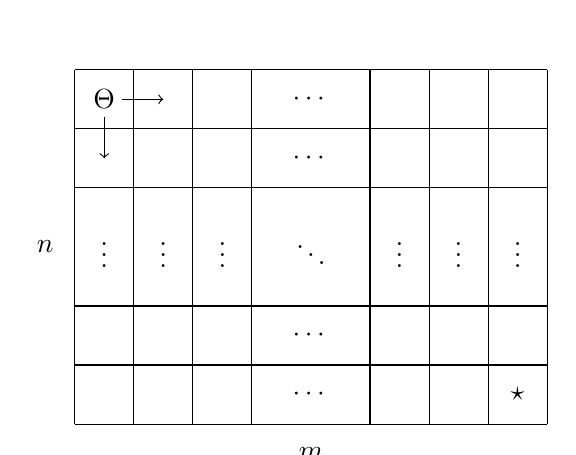
\begin{tikzpicture}[scale=0.75,arrow/.style={->}]
  \foreach \x in {0,1,2,3,5,6,7,8} {
    \draw (\x,0) -- (\x,6);
  }
  \foreach \x in {0.5,1.5,2.5,5.5,6.5,7.5} {
    \node at (\x,3) {$\vdots$};
  }

  \foreach \y in {0,1,2,4,5,6} {
    \draw (0,\y) -- (8,\y);
  }
  \foreach \y in {0.5,1.5,4.5,5.5} {
    \node at (4,\y) {$\cdots$};
  }
  \node at (4,3) {$\ddots$};
  
  \draw[arrow] (0.8,5.5) -- (1.5,5.5);
  \draw[arrow] (0.5,5.2) -- (0.5,4.5);

  \node at (0.5,5.5) {$\Theta$};
  \node at (7.5,0.5) {$\star$};

  \node at (-0.5,3) {$n$};
  \node at (4,-0.5) {$m$};
\end{tikzpicture}
\end{center}
%
The robot starts in cell $(1, 1)$ and can take steps either to the right or down (\textbf{no left or up
steps}). How many distinct paths can the robot take to the destination ($\star$) in cell $(n, m)$ if
    \begin{enumerate}[label=\alph*.]

    \item there are no additional constraints?
    \item the robot must start by moving to the right?
    \item the robot changes direction exactly 3 times? Moving down two times in a
row is not changing directions, but switching from moving down to moving right is. 
For example, moving [down, right, right, down] would count as having two direction changes.

    \end{enumerate}

    \begin{shaded}
    \begin{answer}

    \end{answer}
    \end{shaded}
    \newpage


% 8
\item Say we roll a six-sided die six times. What is the probability that
    \begin{enumerate}[label=\alph*.]
    \item we will roll two different numbers \textit{thrice} (three times) each?
    we will roll \textit{exactly one} number \textit{exactly} three times? Hint: Be careful of overcounting.
    \end{enumerate}

    \begin{shaded}
    \begin{answer}

    \end{answer}
    \end{shaded}
    \newpage


% 9
\item A binary string containing $M$  0's and $N$  1's (in arbitrary order, where all orderings are equally likely) is sent over a network.  What is the probability that the first $r$ bits of the received message contain exactly $k$  1's?

    \begin{shaded}
    \begin{answer}

    \end{answer}
    \end{shaded}
    \newpage


% 10
\item Say we send out a total of 20 distinguishable emails to 12 distinct users, where each email we send is equally likely to go to any of the 12 users (note that it is possible that some users may not actually receive any email from us).  What is the probability that the 20 emails are distributed such that there are 4 users who receive exactly 2 emails each from us and 3 users who receive exactly 4 emails each from us?

    \begin{shaded}
    \begin{answer}

    \end{answer}
    \end{shaded}
    \newpage


% 11
\item Say a hacker has a list of $n$ distinct password candidates, only one of which will successfully log her into a secure system.
    \begin{enumerate}[label=\alph*.]

    \item If she tries passwords from the list at random, deleting those passwords that do not work, what is the probability that her first successful login will be (exactly) on her $k$-th try?
    \item Now say the hacker tries passwords from the list at random, but does \textbf{not} delete previously tried passwords from the list. She stops after her first successful login attempt.  What is the probability that her first successful login will be (exactly) on her $k$-th try?

    \end{enumerate}

    \begin{shaded}
    \begin{answer}

    \end{answer}
    \end{shaded}
    \newpage


% 12
\item Suppose that $m$ strings are hashed (randomly) into $N$ buckets, assuming that all $N^m$ arrangements are equally likely.  Find the probability that exactly $k$ strings are hashed to the first bucket.

    \begin{shaded}
    \begin{answer}

    \end{answer}
    \end{shaded}
    \newpage


% 13
\item \textbf{[Extra credit]} To get good performance when working binary search trees (BST), we must consider the probability of producing completely degenerate BSTs (where each node in the BST has at most one child). See Lecture Notes \# 2, Example 2, for more details on binary search trees.
    \begin{enumerate}[label=\alph*.]

    \item If the integers 1 through $n$ are inserted in arbitrary order into a BST (where each possible order is equally likely), what is the probability (as an expression in terms of $n$) that the resulting BST will have completely degenerate structure?
    \item Using your expression from part (a), determine the smallest value of $n$ for which the probability of forming a completely degenerate BST is less than 0.001 (i.e., 0.1\%).

    \end{enumerate}

    \begin{shaded}
    \begin{answer}

    \end{answer}
    \end{shaded}
    \newpage


% 14
\item \textbf Consider a game, which uses a generator that produces independent random integers between 1 and 100, inclusive. The game starts with a sum $S = 0$. The first player adds random numbers from the generator to $S$ until $S > 100$, at which point they record their last random number \texttt{x}. The second player continues by adding random numbers from the generator to $S$ until $S > 200$, at which point they record their last random number \texttt{y}. The player with the highest number wins; e.g., if \texttt{y} $>$ \texttt{x}, the second player wins. Write a Python 3 program to simulate 100,000 games and output the estimated probability that the second player wins.

    \begin{shaded}
    \begin{answer}
Submit your code to Gradescope. Read the Problem Set handout for more details on submission and the autograder!
    \end{answer}
    \end{shaded}
    \newpage



\end{enumerate}


\end{document}
  
